\chapter{Návrh systému}\label{kap:design}
V~této kapitole je popsán návrh systému pro sběr, zpracování, vyhodnocení a zobrazení dat z~různých senzorů umístěných na průmyslových strojích.

Hlavními požadavky na systém je jeho snadná škálovatelnost, rychlost a modularita. Požadavky vychází ze zkušeností partnerské firmy s~jejich vlastním systémem. Škálovatelností je myšlena možnost rychlého nasazení nových jednotek se senzory a možnost jednoduchého rozšíření výpočetní síly serverové části, aby byla schopná efektivně zpracovávat data od různého množství jednotek. Modularitou systému je míněna možnost snadné výměny jednotlivých částí bez hlubších zásahů do programové části. Například změna úložiště dat, možnosti nasazení různých implementací jednotek, změna komunikačních protokolů a podobně. Systém by také měl být schopný zpracovávat data v~reálném čase a dostupnost uložených dat by měla být okamžitá.

\begin{figure}[h]
  \centering
  \scalebox{0.40}{
        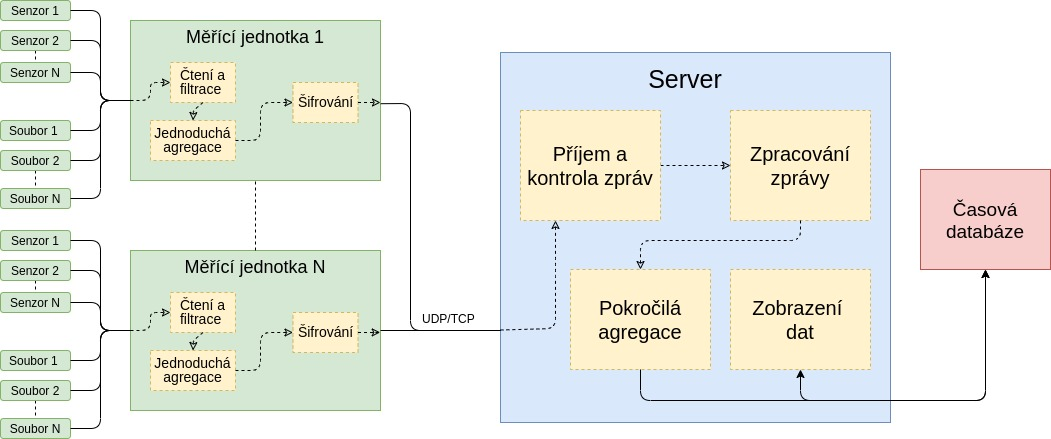
\includegraphics{obrazky-figures/Scalable_platform.jpg}
    }
  \caption{Zjednodušené schéma systému pro sběr, zpracování, vyhodnocení a zobrazení dat.}\label{pic:basic_design}
\end{figure}

Na obrázku \ref{pic:basic_design} je zobrazeno jednoduché schéma navrženého systému. Systém obsahuje měřící jednotky, které čtou data o~pevně nastavené vzorkovací frekvenci z~připojených senzorů, nebo v~případě testování ze souborů. Měřící jednotka kromě čtení provádí filtrování vstupních dat (například snížení vzorkovací frekvence). Vyfiltrovaná data jsou následně agregována jednoduchými, rychlými algoritmy. Po dokončení agregace jsou data zašifrována a pomocí protokolu UDP odesílána na server. Měřící jednotka je též schopná posílat na server neupravené bloky hodnot obsahující důležité úseky měření pro pokročilejší zpracování dat na serveru. Tato data jsou odesílána přes protokol TCP. Data agregovaná na jednotce slouží pro detekci fatálních poruch a sledování vytížení strojů. Tyto hodnoty mohou být využity pro spouštění odesílání nezpracovaných dat. Neagregovaná data zpracovávána serverovou částí neslouží k~detekci poruch, ale jejich predikci. Partnerská firma k~vypracování této práce poskytla software pro zpracování těchto hodnot a prototyp zařízení pro sběr dat ze senzorů vibrací a teploty. Návrh programové části pro měřící jednotku je ovlivněn vlastnostmi tohoto prototypu.

Zprávy přijímá serverová část. O~příjem se starají dva programy -- jeden pro zpracování UDP zpráv obsahující filtrovaná, agregovaná data a druhý pro příjem TCP zpráv s~neupravenými hodnotami. Programy zprávy dešifrují a provedou jejich kontrolu. Bloky neupravených dat jsou ukládány ve formátu TDMS\footnote{tdms -- Technical Data Management Streaming File} na úložiště pro pokročilé zpracování. Soubory slouží i jako záloha. Více informací k~formátu TDMS a účelu těchto dat se nalézá v~sekci \ref{subsec:tcp_server_design}. Hodnoty z~UDP zpráv, které jsou již předzpracované procházejí pokročilou agregací (pokud je to nutné). Následně jsou zapsány do časové databáze. Pokud tyto hodnoty překročí určitou hodnotu je uživatel či správce notifikován.

%popsat tdms soubory a jejich funkci do sekce k tcp serveru

\section{Měřící jednotka}
Měřící jednotka partnerské firmy na které byl vyvíjen software pro sběr a zpracování dat se skládá z~mini počítače Raspberry Pi verze 3b (dále jen RPi) a rozšiřující desky. Partnerskou firmou vyvinutá deska je k~RPi připojena přes GPIO (General-Purpose Input/Output) piny. Deska obsahuje ve starší verzi čtyři vstupy pro senzory vibrací a v~novější verzi i tři konektory pro snímání teploty. Návrh softwaru pro jednotku, jehož schéma je možné vidět na obrázku \ref{pic:unit_design}, je určen právě pro počítač RPi a je ovlivněn jeho parametry. Návrh také počítá s~připojením starší verze desky s~možností připojení čtyř senzorů vibrací, protože novější verze desky nebyla k~dispozici pro testování. Měřící jednotka běží na operačním systému Raspbian, který je linuxovou distribucí speciálně upravenou pro RPi.

RPi bylo zvoleno z~důvodu snadné dostupnosti, nízké ceny, výkonu a hlavně kvůli jeho rozšířenosti a velké komunitě. Pro RPi a linuxovou distribuci Raspbian existuje mnoho knihoven, které usnadňují implementaci komunikace s~připojenými periferiemi přes výstupní piny. 


\subsection{Čtení a filtrování dat}
Hlavní částí návrhu jednotky je program \textit{RawDataParser}, který se skládá ze dvou částí -- procesu pro čtení dat (\textit{Reader}) a procesu pro filtrování dat (\textit{Filter}). Hodnoty ze senzorů vibrací poskytuje analogově digitální převodník ADS131A04 od výrobce Texas Instruments. AD převodník je umístěný na rozšiřující desce a s~RPi komunikuje přes sériové periferní rozhraní (dále jen SPI). Proto program pro čtení dat podporuje komunikaci přes SPI, a z~důvodu testování má i podporu čtení dat ze souboru. AD převodník na desce vzorkuje data ze senzorů o~frekvenci až 128 kHz a proto software \textit{Reader} teoreticky zvládá číst až 512~000 hodnot za vteřinu (128 000 hodnot za vteřinu ze čtyř senzorů). Velikost jedné hodnoty je 24 b. Rozšiřující deska notifikuje RPi o~připravenost dat pro čtení pomocí sestupné hrany signálu pojmenovaném \textit{data ready} na nastaveném pinu. Čtení ze souboru nabízí stejnou možnost získávání dat o~nastavené vzorkovací frekvenci jako přes SPI.

Přečtená data jsou po časových úsecích zapisována do bloků sdílené paměti, ze které je čte filtrovací proces. Bloky jsou dva a vždy dochází k~zápisu do jednoho z~nich a čtení z~druhého. Takto navržené sdílení dat umožní, aby čtecí proces nečekal na uvolnění bloku sdílené paměti a tím nedocházelo ke ztrátě vzorků. Jakmile je časový úsek přečten filtrovacím procesem dojde ke snížení vzorkovací frekvence pomocí filtrů a takto zpracovaná data jsou umístěna do třetího bloku sdílené paměti pro agregační program. Neupravený časový úsek o~původní vzorkovací frekvenci je v~případě potřeby odesílána pomocí protokolu TCP na server pro účely výpočetně náročnějšího zpracování.

Jednotlivé procesy programu \textit{RawDataParser} jsou umístěny na izolovaných jádrech procesoru. Toto rozhodnutí bylo učiněno z~důvodu zvolené platformy a operačního systému. Nejedná se totiž o~\textit{real-time} operační systém. Z~toho důvodu není možné zajistit běh programu v~reálném čase, pokud jsou programy umístěny na jádrech s~více puštěnými procesy. Více k~této problematice se nachází v~\ref{sec:readAndFilter}.
 
\begin{figure}[h]
  \centering
  \scalebox{0.35}{
        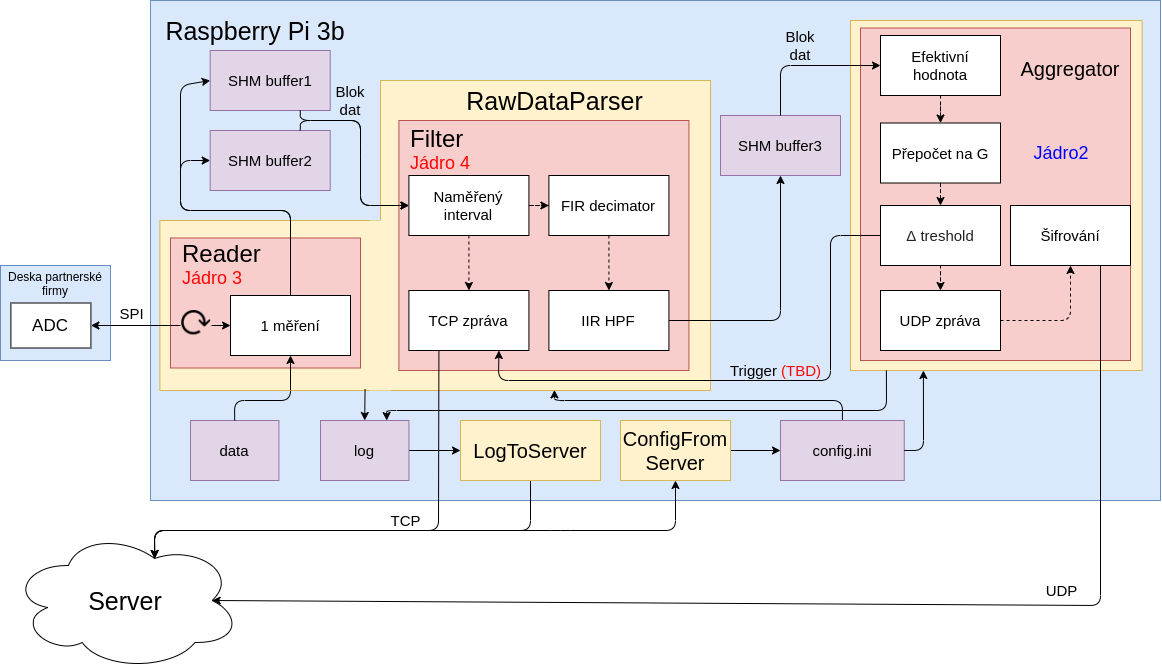
\includegraphics{obrazky-figures/unit.png}
    }
  \caption{Schéma softwaru měřící jednotky.}\label{pic:unit_design}
\end{figure}

\subsection{Agregace dat}
Jak již bylo zmíněno na začátku kapitoly, data agregovaná jednotkou slouží pro zobrazení vytížení stroje a případně i jako indikátor pro odesílání nezpracovaných dat na server. Návrh proto počítá s~triggerem, který upozorňuje filtrovací proces při překročení určité hodnoty. Tato hranice může být nastavena například na zapnutí stroje. Filtrovací proces po upozornění začne odesílat nezpracované bloky dat na server pomocí komunikačního protokolu přes TCP. Funkcionalita triggeru není kritická, ale slouží ke snížení síťové komunikace a potřebné výpočetní síly na serveru. V~případě kdy je sledovaný stroj vypnutý, nebude docházet ke zbytečnému odesílání dat k~pokročilému zpracovávání. Tato funkce ale může být překážkou pro stabilní zpracovávání dat není proto součástí výsledného systému. Nezpracovaná data jsou tedy vždy odesílána na server v~pravidelných intervalech nehledě na stav stroje.

Cílem agregačního programu je redukce dat se sníženou vzorkovací frekvencí předávaných přes sdílenou paměť programem pro čtení a filtrování na zhruba 1-100 vzorků za vteřinu. Toto rozpětí bylo vybráno proto, aby bylo možné zachovat nejdůležitější informace při velkých změnách v~měření. Díky tomu by při běžné činnosti nemělo docházet k~přílišnému zatěžování serverové strany obrovským množstvím hodnot. Za zvážení také stojí omezení zasílání agregovaných dat pokud je stroj nečinný. Neodesílání dat ve vypnutém stavu ale může zamezit sledování stroje v~reálném čase, protože aktualizace hodnot probíhá po delším časovém intervalu.

V~prvním kroku jsou data redukována na 100 vzorků za vteřinu. Tato redukce probíhá pomocí výpočtu kvadratického průměru popsaného v~sekci \ref{sec:vibrationAggregation}. V~dalším kroku dochází k~přepočtu hodnoty na zrychlení $g$ podle vzorce:
\begin{eqnarray}\label{eq:gravity}
  g & = & \frac{x_{out} - x_{rest}}{sensitivity}
\end{eqnarray}
kde $x_{out}$ je výstupní hodnota v~$mV$, $x_{rest}$ je klidová hodnota akcelerometru v~$mV$ a $sensitivity$ je citlivost senzoru v~$mV/g$. Citlivost je dohledatelná v~technické dokumentaci senzorů \cite{accelerationEq}. Po přepočtu na $g$ dochází v~dalším kroku k~zahození hodnot pomocí prahovací funkce hodnoty a času. Ponechány jsou pouze hodnoty, které se liší o~nastavený rozdíl či došlo k~překonání určeného časového intervalu od poslední uložené hodnoty. Po dokončení agregace je z~hodnot poskládána UDP zpráva. Zpráva je zašifrována a odeslána na server. Tato implementace zpracovává data ze senzorů vibrací. Konfigurační soubor ovšem obsahuje položku typ senzoru a v~případě připojení jiných typů senzorů je možné snadno doimplementovat jiný typ přepočtu na fyzikální veličiny či agregace.

%vypocet voltu http://www.ti.com/lit/ds/symlink/ads131a04.pdf


\subsection{Další programy a funkce}
Nejdůležitějším programem jednotky je \textit{RawDataParser} věnující se zpracováním dat. Kromě tohoto programu ovšem jednotka obsahuje i jiné podpůrné programy, skripty a soubory.

\subsubsection*{Instalační skripty}
V~rámci zjednodušení nasazení velkého počtu jednotek za co nejkratší možnou dobu je součástí návrhu sada instalačních skriptů, která automaticky při prvním zapojení inicializuje jednotku. Cílem sady skriptů je, aby pomocí spuštění jednoho skriptu na počítači s~připojenou SD kartou určenou pro RPi došlo k~vytvoření obrazu systému na kartě. Na kartu jsou nakopírovány všechny zbylé instalační skripty a potřebné soubory. Po vložení takto nachystané karty dojde ke kompletní instalaci a inicializaci všech částí softwaru jednotky, a to včetně určení unikátního ID, stáhnutí konfiguračního souboru ze serveru a spuštění samotného měření. Tato inicializace jednotky probíhá automatizovaně bez jakéhokoliv zásahu zvenčí.

\subsubsection*{Konfigurační soubor}
Konfigurační soubor poskytuje možnost jednoduchého nastavení jednotky. Obsahuje veškeré důležité informace pro běh programů a to je:
\begin{itemize}
    \item identifikátor jednotky obsahující unikátní sériové číslo procesoru RPi,
    \item zapnutí zápisu logů, cestu k~souborům s~logy, nastavení odesílání logů na server
    \item zdroj čtení, rychlost čtení, nastavení pinů, cesta k~zálohám a podobně,
    \item parametry pro agregaci hodnot,
    \item nastavení senzorů, jejich piny, zapnutí, citlivost a typ,
    \item IP adresy a porty k~serverům pro odesílání dat.
\end{itemize}
Konfigurační soubor je automaticky stahovaný ze serveru. Informace určené k~časté změně jsou na serveru uložené v~relační databázi jejíž návrh je popsán v~podsekci \ref{subsec:relation_db}. Upravovat pomocí databáze je možné nastavení agregace či parametry senzorů. Nastavení jako cesty k~zálohám či IP adresy serverů je možné změnit jen v~serverové aplikaci pro generování konfiguračního souboru. Jednotka periodicky zjišťuje, zda došlo ke změně konfiguračního souboru. Při změně dochází ke stažení nové konfigurace a restartu jednotky. Aktivní dotazování bylo zvoleno z~toho důvodu, že může nastat situace, kdy jednotku není možné notifikovat z~vnější sítě o~změně parametrů. Soubor má formát .ini. Formát .ini se člení na sekce záznamů a každý záznam obsahuje dvojici klíč, hodnota. Příklad obsahu souboru vypadá takto: 
\lstdefinelanguage{Ini}
{
    basicstyle=\ttfamily\small,
    columns=fullflexible,
    tag=[s]{[]},
    tagstyle=\color{blue}\bfseries,
    usekeywordsintag=true,
    morecomment=[l]{;},
    commentstyle=\color{gray}\ttfamily,
    alsoletter={=},
    ndkeywords={=},
    ndkeywordstyle=\color{green}\bfseries
}[html]
 \begin{lstlisting}[language={Ini}]
    ;aggreagation parameters
    [aggregation]
    delta = 10.2
    average = 80

    #server parameters
    [server]
    udp_ip: 255.255.255.255
    udp_port: 42
    \end{lstlisting}

\subsubsection*{Logování}
Chybové výstupy všech programů jsou ukládány do logovacích souborů. Logovací soubory jsou odesílány na server. Záznamy jsou ukládány v~následujícím formátu: \textit{[<časová značka>] [<název programu>] [<stav>] <zpráva>} Příkladem takového záznamu je: \textit{[2020-01-29 14:58:21.227] [Reader] [error] Unable to parse config file: missing frequency value}
%\subsection{Shrnutí návrhu jednotky a požadavky}
%ANO NEBO NE?

\section{Komunikační protokoly}\label{sec:comm_protocol}
UDP protokol je určený ke sledování dat s~co nejmenším možným zpožděním. To znamená časté zasílání menšího množství již agregovaných dat připravených k~přímému zápisu do databáze. Ztráta paketu nemá vliv na systém. Komunikační protokol je zobrazen na obrázku číslo \ref{pic:udp_protocol}. Protokol obsahuje verzi, unikátní identifikátor jednotky, časovou značku začátku měření a počet senzorů v~datové části. Hlavička senzoru je dlouhá 32 bitů. ID senzoru číslované od $0$ označuje index připojeného senzoru. Typ dat označuje jakým způsobem byla data zpracována a určuje do jaké databáze jsou vložena. Velikost označuje počet bajtů za hlavičkou senzoru obsahující hodnoty. Verze protokolu vyjadřuje v~jakém formátu jsou hodnoty odesílány. Maximální délka paketu byla zvolena 512 bajtů, což je minimální délka \textbf{datového bloku} paketu, kterou musí umět každé síťové zařízení zpracovat \cite{rfc791}. 

\begin{figure}[h]
\centering
\begin{subfigure}{.5\textwidth}
  \centering
    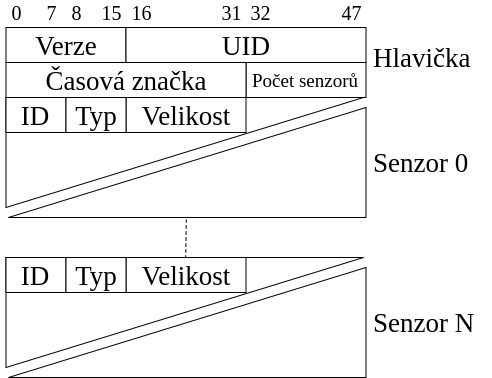
\includegraphics[width=.9\linewidth]{obrazky-figures/udp_paket.png}
    \caption{Schéma UDP paketu.}
  \label{pic:udp_protocol}
\end{subfigure}
\begin{subfigure}{.5\textwidth}
  \centering
    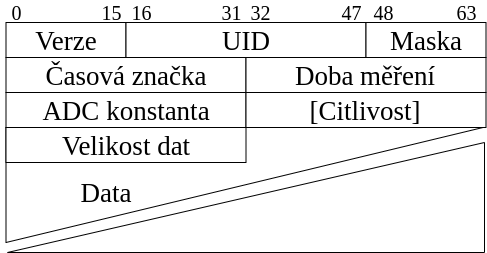
\includegraphics[width=.9\linewidth]{obrazky-figures/tcp_paket.png}
    \caption{Schéma TCP paketu.}
  \label{pic:tcp_protocol}
\end{subfigure}
\caption{Komunikační protokoly.}
\label{fig:test}
\end{figure}

Komunikační protokol založený na TCP slouží k~odeslání časového úseku nezpracovaných dat na pokročilé zpracování. Paket obsahuje oproti UDP zprávě navíc dobu měření ve vteřinách, ADC konstantu pro přepočet hodnot a pole citlivostí jednotlivých senzorů obsažených ve zprávě.



\section{Návrh serveru}
Serverová část systému je navržena tak, aby mohla fungovat pouze z~jednoho fyzického zařízení. V~případě potřeby je ovšem možné jednotlivé programy distribuovat na více serverů. Blokové schéma se nachází na obrázku \ref{pic:server_design}. Návrh obsahuje:
\begin{itemize}
    \item aplikace UDP a TCP serveru,
    \item relační databázi pro správu informací o~jednotkách,
    \item časovou databázi pro ukládání zpracovaných naměřených hodnot,
    \item datové úložiště pro zálohování nezpracovaných úseků měření ve formě TDMS souborů
    \item algoritmy partnerské firmy pro pokročilé zpracování TDMS souborů
    \item webovou aplikaci pro zobrazení grafů z~časové databáze
    \item program pro generování konfiguračních souborů z~databáze
    \item program pro přesměrování datového toku mezi více serverů.
\end{itemize}
Jednotlivé části návrhu jsou detailněji popsány v~následujících podsekcích. 

\begin{figure}[h]
  \centering
  \scalebox{0.44}{
        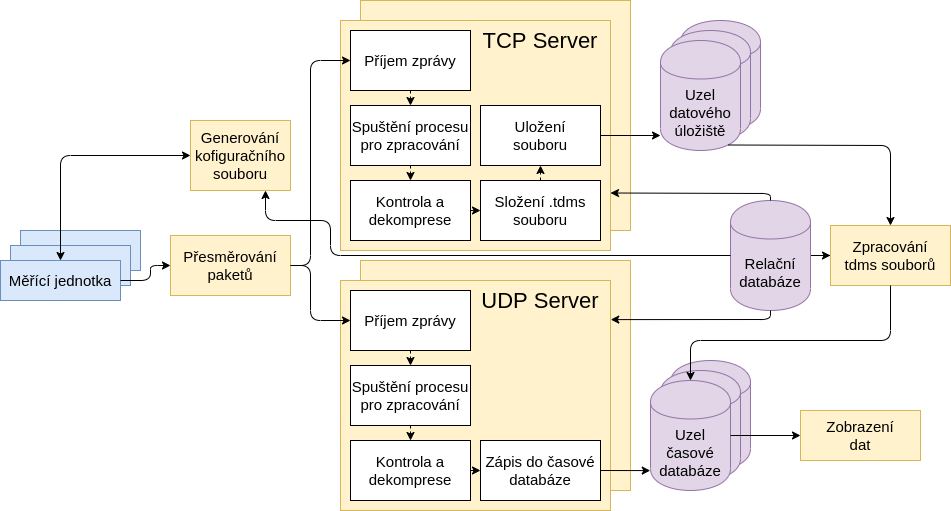
\includegraphics{obrazky-figures/server_design.png}
    }
  \caption{Schéma návrhu serverových aplikací a úložišť.}\label{pic:server_design}
\end{figure}

\subsection{UDP server}
Aplikace slouží pro příjem UDP zpráv obsahující zpracovaná data určená k~zápisu do časové databáze. Při příchodu zprávy dochází k~načtení verze protokolu a UID jednotky. Po načtení informací dochází k~dešifrování obsahu zprávy a k~zápisu hodnot do příslušných sérií v~časové databázi. Aplikace musí být schopna zpracovávat velké množství zpráv v~krátkém časovém úseku, po přijetí každé zprávy proto dochází ke spuštění nového procesu či vlákna, jehož účelem je zpracování zprávy.

\subsection{TCP server}\label{subsec:tcp_server_design}
Zasílání neupravených dat se děje z~důvodu, že RPi nemá dostatečný výkon pro aplikování pokročilých analýz nad daty o~vysoké vzorkovací frekvenci. Data agregovaná na jednotce jsou schopna detekovat poruchu při velké změně hodnot, ale právě agregací se ztrácí informace, které mohou indikovat blížící se poruchu. TCP server slouží k~přijímání bloků těchto dat a jejich zapsání do souborů ve formátu TDMS a uložení na datové úložiště. Formát byl zvolen z~důvodu využití aplikace partnerské firmy pro pokročilé zpracování dat. Tato aplikace je vytvořena v~programu LabView a vstupem jsou právě soubory ve formátu TDMS.

\subsection{Relační databáze}\label{subsec:relation_db}
Jednoduchá relační databáze slouží pro správu a nastavení jednotek, senzorů a přehled monitorovaných strojů. Schéma databáze je vidět na obrázku \ref{pic:relation_design}. Databáze obsahuje tabulky se společnostmi, jimi vlastněnými stroji a komponenty jednotlivých strojů. Senzory jsou připojené ke komponentům a tabulka senzorů obsahuje informaci o~citlivosti a zda je senzor zapojen. Senzory přísluší k~měřící jednotce, tabulka jednotky obsahuje zbylé informace potřebné pro vygenerování konfiguračního souboru.

\begin{figure}[h]
  \centering
  \scalebox{0.53}{
        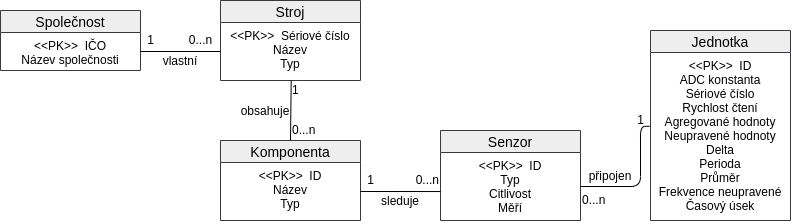
\includegraphics{obrazky-figures/Database.png}
    }
  \caption{Schéma návrhu relační databáze.}\label{pic:relation_design}
\end{figure}

\subsection{Časová databáze}
Tento typ úložiště slouží k~ukládání naměřených zpracovaných dat. Schéma na obrázku \ref{pic:time_series_design} obsahuje jednu databázi pro každou jednotku, jejíž název je unikátní ID jednotky. Jednotlivé databáze obsahují samotné časové série. Jméno časové série je odvozeno podle čísla senzoru, kterým byly hodnoty naměřeny, a podle způsobu, kterým byly zpracovány. Záznam je kombinací hodnoty a času. Pro zobrazování hodnot je využito grafické rozhraní zvolené databáze.

\begin{figure}[h]
  \centering
  \scalebox{0.60}{
        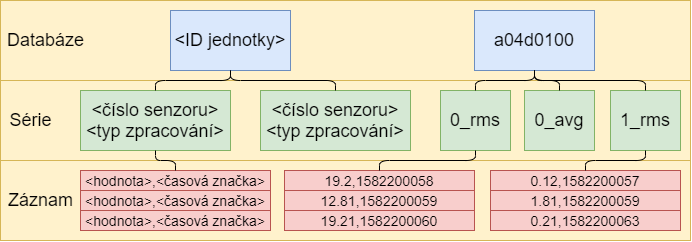
\includegraphics{obrazky-figures/time_series_design.png}
    }
  \caption{Schéma rozložení dat v~časové databázi.}\label{pic:time_series_design}
\end{figure}

\subsection{Ostatní programy a funkcionalita}
Součástí návrhu je program pro přesměrování paketů. Tento program umožňuje připojení více instancí TCP a UDP serverů. Pro tuto funkcionalitu je zvoleno již existující volně dostupné řešení a jeho využití v~systému je řešeno v~rámci testování. 

Další součástí je generování konfiguračního souboru. Program při zadání identifikátoru jednotky provede vygenerování konfigurace do souboru v~místě spuštění. Konfigurace jsou následně jednotkami staženy přes HTTP dotaz.
